\section{Introduction}

Transformer-based models~\cite{transformer-nips17,qwen2-5-arxiv25,deepseek-v3-arxiv25,llama3-arxiv24} have demonstrated remarkable capabilities in multimodal understanding, reasoning, and generation, establishing themselves as foundational architectures for next-generation large multimodal models (LMMs)~\cite{qwen2.5-vl-arxiv25,gpt4o-arxiv24,llama3-arxiv24,step-audio-arxiv25,step-t2v-arxiv25,gemini-3-2025}. Modern LMMs integrate multiple \emph{modality modules}, including encoders, decoders, and backbone models connected via modality adapters. This architectural design enables flexible and seamless processing of interleaved multimodal data (\eg text, images, video), thereby supporting diverse task paradigms such as multimodal document understanding~\cite{mlongdoc-arxiv24} and multi-turn dialogs~\cite{gpt4o-image-generation}.

However, this architectural flexibility introduces significant challenges in training due to irregular and fluctuating execution latencies across different modality modules and data batches, leading to a unique problem of \emph{dynamic imbalance}. This challenge stems from two interrelated factors:

\textbf{Pipeline Stage Imbalance:}
LMMs exhibit architectural heterogeneity arising from diverse modality modules with distinct parameter shapes and operator types (\eg attention, GEMM, convolution). These differences create skewed computational workloads and varying memory access patterns, complicating the partitioning of model execution into balanced pipeline stages.
Even with exhaustive enumeration of all possible layer splits, the ``optimal'' partitioning still incurs a 22.8\% pipeline bubble overhead for a 37B-parameter LMM (\S\ref{section:impact-on-pipeline-parallelism}).
This inefficiency is primarily due to the significant discrepancy between heterogeneous layers, which prevents perfectly balanced pipeline stage partitioning.

\textbf{Training Data Dynamicity:}
The inherent architectural heterogeneity is further exacerbated by the diversity of multimodal training data, which comprises large-scale datasets with highly variable modality distributions across batches.
% This dynamicity renders the conventional approach of using a single, static pipeline schedule infeasible for LMM training.
Although data packing techniques~\cite{wlb-llm-osdi25,dynapipe-eurosys24} aim to produce more balanced batches, computational imbalance persists. In our experiments, the largest data sample incurs $4.15\times$ greater computational load than the smallest (\S\ref{section:dynamic-imbalance}). Such disparities cause substantial workload fluctuations between batches.

The combination of pipeline stage imbalance and training data dynamicity results in a significant performance bottleneck. Our experiments show that this dynamic imbalance can inflate training overhead by up to 40.3\% for the 37B LMM (\S\ref{section:impact-on-pipeline-parallelism}).
This performance degradation renders the conventional approach of using a single, static pipeline schedule (\eg Megatron-LM's 1F1B) impractical and inefficient for the dynamic nature of LMMs.
% Megatron-LM~\cite{megatron-lm-arxiv20}, the state-of-the-art framework for training unimodal LLMs with homogeneous transformer layers, employs a static 1F1B pipeline schedule and is inadequate for heterogeneous modality modules.
Similarly, training systems for multimodal models such as Spindle~\cite{spindle-asplos25} and Optimus~\cite{optimus-atc25} rely on static pipeline schedules tailored for a fixed set of tasks.
Their training plans are determined before training start, overlooking the dynamic nature of multimodal data and resulting in suboptimal pipeline performance.
Existing approaches~\cite{wlb-llm-osdi25,dynapipe-eurosys24,flexpipe-atc25} designed for dynamic text sequence lengths are also insufficient.
They primarily address workload variations that affect all layers of a unimodal LLM uniformly.
However, they cannot resolve the fundamental inter-modality imbalance in LMMs,
where a change in one modality (\eg more images) can drastically overload a specific module while leaving others underutilized.

To address these challenges, we propose \sys{}, a dynamic and modality-aware scheduling framework designed to optimize pipeline parallelism for LMMs. \sys{} is built upon two key insights that identify the root causes of pipeline inefficiency.
First, co-locating computations from different modality modules within the same pipeline execution pass is inherently inefficient due to their disparate computational costs (\figref{figure:schedule-observations}a).
We define a \emph{pipeline segment} as a complete forward or backward pass of computations across all pipeline stages.
To eliminate this \emph{intra-segment imbalance}, \sys{} enforces separated partitioning, dedicating distinct pipeline segments to each modality (\figref{figure:schedule-observations}b).
This isolation prevents slow modalities from bottlenecking faster ones.
Second, even after separation, workload imbalances persist between these modality-specific segments.
To resolve this \emph{inter-segment imbalance}, \sys{} further dynamically splits data into smaller, modality-specific \emph{sub-microbatches} (\figref{figure:schedule-observations}c).
This modality-aware partitioning approach allows latencies of different modality segments to be more closely matched,
resulting in finer-grained load balancing between these segments.

\begin{figure}[!t]
    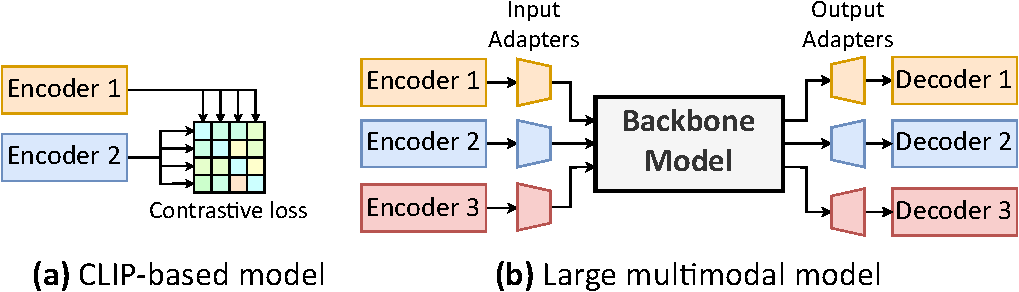
\includegraphics[width=1\columnwidth]{./figures/svg/mm_vs_lmm.pdf}
    \caption{
        Comparison between CLIP-based models and LMMs.
    }
    \label{figure:mm-vs-lmm}
\end{figure}

\begin{figure}[!t]
    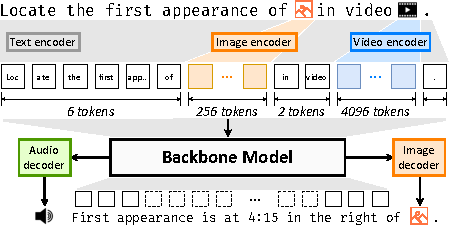
\includegraphics[width=1\columnwidth]{./figures/svg/mllm_demo.pdf}
    \caption{
        An example of LMM that uses a large language model as the backbone.
        The user prompt consists of an image and a video clip,
        and is converted into tokens by corresponding modality encoders,
        which are further processed by the backbone model to produce the response
        in multimodal text or speech audio.
    }
    \label{figure:mllm-demo}
\end{figure}

Meanwhile, in contrast to conventional systems that rely on static or pre-computed schedules, \sys{} employs asynchronous schedule generation. It generates a custom pipeline schedule for each data batch on-the-fly, seamlessly adapting to the fluctuating computational demands of multimodal data.
To avoid stalling training, \sys{} generates schedules using idle CPU cores in parallel with the main GPU training workers, effectively hiding search latency.
To identify high-quality schedules within the tight time constraints of a training iteration (typically 10--60 seconds), \sys{} decomposes the complex search problem into three simpler subproblems,
each with a tailored heuristic to reduce search space.
\sys{} parallelizes the search loop over hundreds of CPU cores, shortening the search time and harnessing idle CPUs.

We implement \sys{} on top of Megatron-LM, the state-of-the-art distributed training framework for transformer-based large language models. In addition to the scheduling algorithms, we develop a training simulator for fast and accurate prediction of pipeline stage latency and memory consumption. We also enhance Megatron-LM with a reconfigurable pipeline mechanism to support dynamic pipeline schedule deployment.
We validate \sys{} on a diverse set of five LMMs, ranging from 12B to 94B parameters and including vision-language models and diffusion models.
Experimental results demonstrate that \sys{} achieves up to 97.3\% higher training performance compared to baseline systems.
Moreover, \sys{} exhibits excellent adaptability to the dynamic workloads of LMM training, maintaining near-optimal hardware utilization throughout the training process.

In summary, this paper makes the following contributions:

\begin{itemize}
    \item We identify and characterize the problem of dynamic imbalance in LMM training, a challenge arising from the interplay between pipeline stage imbalance and training data dynamicity.
    \item We propose \sys{}, a novel scheduling framework that employs asynchronous schedule generation, modality-aware partitioning, and a decomposed search algorithm to dynamically adapt to varying workloads.
    \item We evaluate \sys{} against three state-of-the-art training systems across five LMM models up to 94B, demonstrating improvements of up to 97.3\% in training efficiency.
\end{itemize}
